\tikzstyle{line} = [draw]

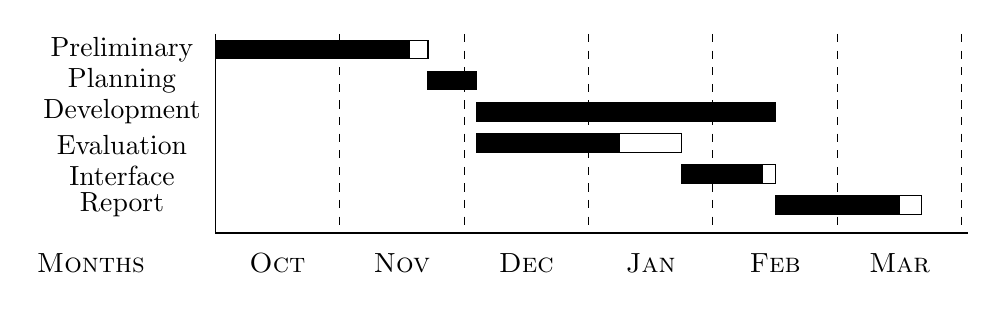
\begin{tikzpicture}[scale=0.79]
%\draw[help lines] (0,0) grid +(10,1);
%lines
\draw (0,0) -- (0,-3.2);
%\path [line,dashed] (1,0) -- (1,-5.7);
\path [line,dashed] (2,0) -- (2,-3.2);
%\path [line,dashed] (3,0) -- (3,-5.7);
\path [line,dashed] (4,0) -- (4,-3.2);
%\path [line,dashed] (5,0) -- (5,-5.7);
\path [line,dashed] (6,0) -- (6,-3.2);
%\path [line,dashed] (7,0) -- (7,-5.7);
\path [line,dashed] (8,0) -- (8,-3.2);
%\path [line,dashed] (9,0) -- (9,-5.7);
\path [line,dashed] (10,0) -- (10,-3.2);
%\path [line,dashed] (11,0) -- (11,-5.7);
\path [line,dashed] (12,0) -- (12,-3.2);

\draw (-1.5,-0.6) node[above]{Preliminary};%
\draw (-1.5,-1.1) node[above]{Planning};%
\draw (-1.5,-1.6) node[above]{Development};%
\draw (-1.5,-2.1) node[above]{Evaluation};%
\draw (-1.5,-2.6) node[above]{Interface};%
\draw (-1.5,-3.1) node[above]{Report};%
%\draw (-1.5,-3.5) node[above]{$ \textsc{activity G}$};%
%\draw (-1.5,-4) node[above]{$ \textsc{activity H}$};%
%\draw (-1.5,-4.5) node[above]{$ \textsc{activity I}$};%
%\draw (-1.5,-5) node[above]{$ \textsc{activity J}$};%
%\draw (-1.5,-5.5) node[above]{$ \textsc{Report}$};%

\filldraw[fill=white] (0,-0.1) rectangle (3.42,-0.4);% a slack
\filldraw[fill=black] (0,-0.1) rectangle (3.12,-0.4);% a
\filldraw[fill=white] (3.42,-0.6) rectangle (4.2,-0.9);% b slack
\filldraw[fill=black] (3.42,-0.6) rectangle (4.2,-0.9);% b
\filldraw[fill=black] (4.2,-1.1) rectangle (9,-1.4);% c
\filldraw[fill=white] (4.2,-1.6) rectangle (7.5,-1.9);% d slack
\filldraw[fill=black] (4.2,-1.6) rectangle (6.5,-1.9);% d
\filldraw[fill=white] (7.5,-2.1) rectangle (9,-2.4);% e slack
\filldraw[fill=black] (7.5,-2.1) rectangle (8.8,-2.4);% e
\filldraw[fill=white] (9,-2.6) rectangle (11.36,-2.9);% k slack
\filldraw[fill=black] (9,-2.6) rectangle (11,-2.9);% k
%\filldraw[fill=white] (3.2,-2.6) rectangle (6.66,-2.9);% f slack
%\filldraw[fill=black] (3.2,-2.6) rectangle (3.4,-2.9);% f
%\filldraw[fill=white] (7,-3.1) rectangle (9.6,-3.4);% g slack
%\filldraw[fill=black] (7,-3.1) rectangle (8,-3.4);% g
%\filldraw[fill=white] (7,-3.6) rectangle (7.53,-3.9);% h slack
%\filldraw[fill=black] (7,-3.6) rectangle (7.43,-3.9);% h 
%\filldraw[fill=black] (6.66,-4.1) rectangle (7.53,-4.4);% i 
%\filldraw[fill=black] (7.53,-4.6) rectangle (9.58,-4.9);% i 

\draw (0,-3.2) -- (12,-3.2);
\draw (0,-3.2) -- (12.1,-3.2);


\draw (-2,-4) node[above]{$ \textsc{Months}$};%
\draw (1,-4) node[above]{$ \textsc{Oct}$};%
%\draw (1,-6.5) node[above]{$ \textsc{21}$};%
\draw (3,-4) node[above]{$ \textsc{Nov}$};%
%\draw (3,-6.5) node[above]{$ \textsc{23}$};%
\draw (5,-4) node[above]{$ \textsc{Dec}$};%
%\draw (5,-6.5) node[above]{$ \textsc{25}$};%
\draw (7,-4) node[above]{$ \textsc{Jan}$};%
%\draw (7,-6.5) node[above]{$ \textsc{27}$};%
\draw (9,-4) node[above]{$ \textsc{Feb}$};%
%\draw (9,-6.5) node[above]{$ \textsc{29}$};%
\draw (11,-4) node[above]{$ \textsc{Mar}$};%
%\draw (11,-6.5) node[above]{$ \textsc{31}$};%
%\draw (12,-6.5) node[above]{$ \textsc{}$};%
\end{tikzpicture}


